\documentclass[11pt,a4paper]{article}
\usepackage[utf8]{inputenc}
\usepackage[T1]{fontenc}
\usepackage[english]{babel}
\usepackage{geometry}
\usepackage{amsmath}
\usepackage{amsfonts}
\usepackage{amssymb}
\usepackage{graphicx}
\usepackage{xcolor}
\usepackage{hyperref}
\usepackage{listings}
\usepackage{fancyhdr}
\usepackage{titlesec}
\usepackage{tcolorbox}
\usepackage{enumitem}
\usepackage{booktabs}
\usepackage{array}
\usepackage{multicol}
\usepackage{tikz}
\usepackage{pgfplots}

% Configuration de la page
\geometry{left=2cm,right=2cm,top=2.5cm,bottom=2.5cm}

% Configuration des couleurs
\definecolor{jupiterBlue}{RGB}{59, 130, 246}
\definecolor{solanaGreen}{RGB}{34, 197, 94}
\definecolor{deauraPurple}{RGB}{168, 85, 247}
\definecolor{codeGray}{RGB}{248, 250, 252}
\definecolor{warningOrange}{RGB}{251, 146, 60}
\definecolor{successGreen}{RGB}{16, 185, 129}

% Configuration des liens
\hypersetup{
    colorlinks=true,
    linkcolor=jupiterBlue,
    filecolor=jupiterBlue,
    urlcolor=jupiterBlue,
    citecolor=jupiterBlue
}

% Configuration des listings
\lstdefinestyle{typescript}{
    language=JavaScript,
    backgroundcolor=\color{codeGray},
    basicstyle=\ttfamily\footnotesize,
    breakatwhitespace=false,
    breaklines=true,
    captionpos=b,
    commentstyle=\color{solanaGreen},
    deletekeywords={...},
    escapeinside={\%*}{*)},
    extendedchars=true,
    frame=single,
    keepspaces=true,
    keywordstyle=\color{jupiterBlue},
    morekeywords={interface,type,const,let,async,await,export,import,from,as,extends,implements},
    numbers=left,
    numbersep=5pt,
    numberstyle=\tiny\color{gray},
    rulecolor=\color{black},
    showspaces=false,
    showstringspaces=false,
    showtabs=false,
    stepnumber=1,
    stringstyle=\color{deauraPurple},
    tabsize=2,
    title=\lstname
}

% Configuration des titres
\titleformat{\section}{\Large\bfseries\color{jupiterBlue}}{\thesection}{1em}{}
\titleformat{\subsection}{\large\bfseries\color{jupiterBlue}}{\thesubsection}{1em}{}
\titleformat{\subsubsection}{\normalsize\bfseries\color{jupiterBlue}}{\thesubsubsection}{1em}{}

% En-tête et pied de page
\pagestyle{fancy}
\fancyhf{}
\fancyhead[L]{\textcolor{jupiterBlue}{\textbf{Jupiter Swap DApp - Complete Architecture Guide}}}
\fancyhead[R]{\textcolor{jupiterBlue}{\textbf{Technical Documentation}}}
\fancyfoot[C]{\thepage}

\begin{document}

% Page de titre
\begin{titlepage}
    \centering
    \vspace*{1cm}
    
    {\Huge\textbf{\textcolor{jupiterBlue}{Complete Project Architecture}}\par}
    \vspace{0.5cm}
    {\LARGE\textcolor{deauraPurple}{Jupiter Swap DApp}\par}
    \vspace{0.3cm}
    {\Large\textit{Technical Guide}\par}
    
    \vspace{1.5cm}
    
    \begin{tcolorbox}[colback=jupiterBlue!10,colframe=jupiterBlue,width=0.9\textwidth]
        \centering
        \textbf{🏗️ Comprehensive Architecture Documentation}\\
        \vspace{0.5cm}
        \begin{multicols}{2}
        \textbf{Frontend:} Next.js 14 + TypeScript\\
        \textbf{Blockchain:} Solana + Jupiter API v6\\
        \textbf{State Management:} Zustand + React Query\\
        \textbf{UI Framework:} Tailwind + shadcn/ui\\
        \textbf{Testing:} Jest + Testing Library\\
        \textbf{Deployment:} Vercel + GitHub Actions\\
        \textbf{Monitoring:} Sentry + Custom Analytics\\
        \textbf{Security:} Multi-layer Protection
        \end{multicols}
    \end{tcolorbox}
    
    \vspace{1.5cm}
    
    \begin{tcolorbox}[colback=solanaGreen!10,colframe=solanaGreen,width=0.8\textwidth]
        \centering
        \textbf{📋 Documentation Coverage}\\
        \vspace{0.3cm}
        ✅ Component Hierarchy \& Design Patterns\\
        ✅ Service Layer Architecture\\
        ✅ State Management Strategy\\
        ✅ API Integration Patterns\\
        ✅ Security Implementation\\
        ✅ Performance Optimization\\
        ✅ Testing Architecture\\
        ✅ Deployment Pipeline
    \end{tcolorbox}
    
    \vfill
    
    {\large\textbf{Author:} Kamel (\href{https://x.com/treizeb__}{@treizeb\_\_})\\
    \textbf{Company:} \href{https://deaura.io}{DeAura.io}\\
    \textbf{Updated:} July 14, 2025\par}
\end{titlepage}

\newpage
\tableofcontents
\newpage

\section{🎯 Architecture Overview}

\subsection{System Architecture Diagram}

\begin{center}
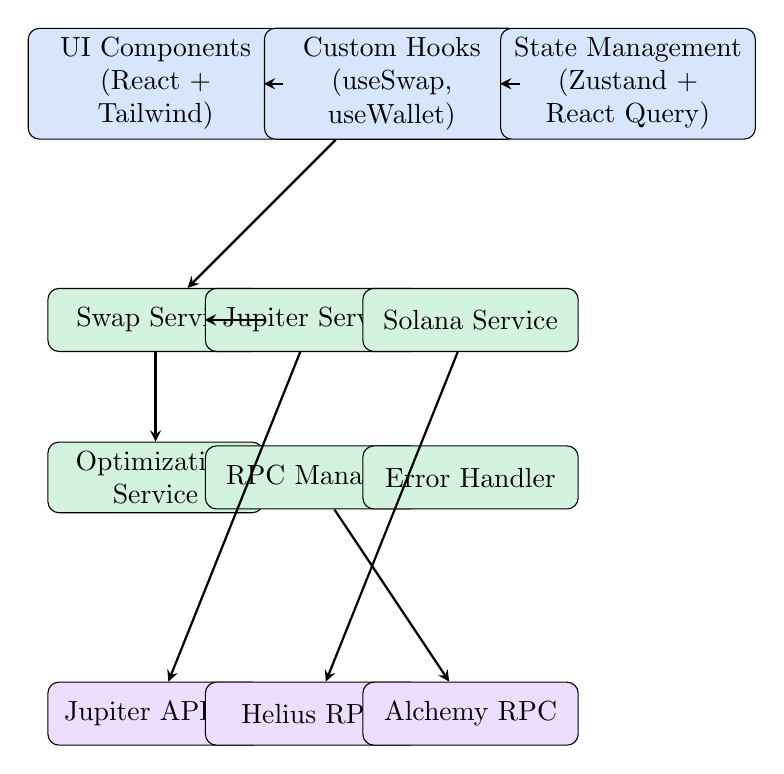
\begin{tikzpicture}[node distance=2cm, auto]
    % Define styles
    \tikzstyle{component} = [rectangle, draw, fill=jupiterBlue!20, text width=3cm, text centered, rounded corners, minimum height=1cm]
    \tikzstyle{service} = [rectangle, draw, fill=solanaGreen!20, text width=2.5cm, text centered, rounded corners, minimum height=0.8cm]
    \tikzstyle{external} = [rectangle, draw, fill=deauraPurple!20, text width=2.5cm, text centered, rounded corners, minimum height=0.8cm]
    \tikzstyle{arrow} = [thick,->,>=stealth]
    
    % Frontend Layer
    \node [component] (ui) {UI Components\\(React + Tailwind)};
    \node [component, right of=ui, xshift=1cm] (hooks) {Custom Hooks\\(useSwap, useWallet)};
    \node [component, right of=hooks, xshift=1cm] (store) {State Management\\(Zustand + React Query)};
    
    % Service Layer
    \node [service, below of=ui, yshift=-1cm] (swap) {Swap Service};
    \node [service, right of=swap] (jupiter) {Jupiter Service};
    \node [service, right of=jupiter] (solana) {Solana Service};
    \node [service, below of=swap] (optimization) {Optimization\\Service};
    \node [service, right of=optimization] (rpc) {RPC Manager};
    \node [service, right of=rpc] (errors) {Error Handler};
    
    % External Services
    \node [external, below of=optimization, yshift=-1cm] (jupiterapi) {Jupiter API v6};
    \node [external, right of=jupiterapi] (helius) {Helius RPC};
    \node [external, right of=helius] (alchemy) {Alchemy RPC};
    
    % Arrows
    \draw [arrow] (ui) -- (hooks);
    \draw [arrow] (hooks) -- (store);
    \draw [arrow] (hooks) -- (swap);
    \draw [arrow] (swap) -- (jupiter);
    \draw [arrow] (swap) -- (optimization);
    \draw [arrow] (jupiter) -- (jupiterapi);
    \draw [arrow] (solana) -- (helius);
    \draw [arrow] (rpc) -- (alchemy);
\end{tikzpicture}
\end{center}

\subsection{Architecture Principles}

\begin{tcolorbox}[colback=jupiterBlue!10,colframe=jupiterBlue]
\textbf{🎯 Core Principles:}
\begin{enumerate}
    \item \textbf{Separation of Concerns:} Clear boundaries between UI, business logic, and data layers
    \item \textbf{Modularity:} Loosely coupled, highly cohesive components
    \item \textbf{Scalability:} Designed to handle increased load and feature expansion
    \item \textbf{Maintainability:} Clean code with comprehensive documentation
    \item \textbf{Testability:} Architecture supports comprehensive testing strategies
    \item \textbf{Performance:} Optimized for speed and efficiency
    \item \textbf{Security:} Multi-layer security implementation
    \item \textbf{Reliability:} Robust error handling and failover mechanisms
\end{enumerate}
\end{tcolorbox}

\section{🧩 Component Hierarchy}

\subsection{Frontend Component Structure}

\begin{lstlisting}[style=typescript, caption=Component Hierarchy Tree]
src/components/
├── providers/
│   ├── Providers.tsx              # Root providers wrapper
│   ├── WalletProvider.tsx         # Solana wallet integration
│   ├── QueryProvider.tsx         # React Query setup
│   └── ThemeProvider.tsx         # Theme management
├── layout/
│   ├── Header.tsx                 # Application header
│   ├── Footer.tsx                 # Application footer
│   ├── Navigation.tsx             # Main navigation
│   └── Sidebar.tsx                # Optional sidebar
├── swap/
│   ├── SwapInterface.tsx          # Main swap component
│   ├── TokenSelector.tsx          # Token selection dropdown
│   ├── AmountInput.tsx            # Amount input with validation
│   ├── SwapButton.tsx             # Swap execution button
│   ├── QuoteDisplay.tsx           # Quote information display
│   ├── SlippageSettings.tsx       # Slippage configuration
│   └── TransactionStatus.tsx      # Transaction progress
├── wallet/
│   ├── WalletConnectButton.tsx    # Wallet connection
│   ├── WalletInfo.tsx             # Wallet information display
│   ├── BalanceDisplay.tsx         # Token balances
│   └── DisconnectButton.tsx       # Wallet disconnection
├── analytics/
│   ├── NetworkStatus.tsx          # Network health indicator
│   ├── OptimizationPanel.tsx      # Optimization settings
│   ├── TransactionHistory.tsx     # Transaction history
│   ├── PerformanceMetrics.tsx     # Performance dashboard
│   └── FeeAnalytics.tsx           # Fee analysis
├── ui/                            # shadcn/ui components
│   ├── button.tsx                 # Button component
│   ├── card.tsx                   # Card component
│   ├── input.tsx                  # Input component
│   ├── dialog.tsx                 # Dialog/Modal component
│   ├── toast.tsx                  # Toast notifications
│   ├── progress.tsx               # Progress indicators
│   ├── tabs.tsx                   # Tab component
│   ├── tooltip.tsx                # Tooltip component
│   ├── select.tsx                 # Select dropdown
│   ├── badge.tsx                  # Badge component
│   ├── separator.tsx              # Separator component
│   └── scroll-area.tsx            # Scroll area
└── errors/
    ├── ErrorBoundary.tsx          # React error boundary
    ├── ErrorDisplay.tsx           # Error message display
    └── FallbackComponent.tsx      # Fallback UI component
\end{lstlisting}

\subsection{Component Design Patterns}

\subsubsection{Compound Component Pattern}

\begin{lstlisting}[style=typescript, caption=SwapInterface Compound Component]
// SwapInterface.tsx - Main compound component
export function SwapInterface() {
  return (
    <SwapProvider>
      <Card className="w-full max-w-md mx-auto">
        <SwapInterface.Header />
        <SwapInterface.Body>
          <SwapInterface.TokenInput type="input" />
          <SwapInterface.SwapButton />
          <SwapInterface.TokenInput type="output" />
        </SwapInterface.Body>
        <SwapInterface.Footer />
      </Card>
    </SwapProvider>
  );
}

// Compound component parts
SwapInterface.Header = function SwapHeader() {
  return (
    <CardHeader>
      <CardTitle>Swap Tokens</CardTitle>
      <CardDescription>
        Exchange SOL and USDC with optimized rates
      </CardDescription>
    </CardHeader>
  );
};

SwapInterface.Body = function SwapBody({ children }: { children: React.ReactNode }) {
  return (
    <CardContent className="space-y-4">
      {children}
    </CardContent>
  );
};

SwapInterface.TokenInput = function TokenInput({ type }: { type: 'input' | 'output' }) {
  const { inputToken, outputToken, inputAmount, outputAmount } = useSwap();
  
  return (
    <div className="space-y-2">
      <Label>{type === 'input' ? 'From' : 'To'}</Label>
      <div className="flex space-x-2">
        <TokenSelector 
          selectedToken={type === 'input' ? inputToken : outputToken}
          onSelectToken={type === 'input' ? setInputToken : setOutputToken}
        />
        <AmountInput
          value={type === 'input' ? inputAmount : outputAmount}
          onChange={type === 'input' ? setInputAmount : undefined}
          readOnly={type === 'output'}
        />
      </div>
    </div>
  );
};

SwapInterface.SwapButton = function SwapButton() {
  const { canSwap, isLoading, executeSwap } = useSwap();
  
  return (
    <Button
      onClick={executeSwap}
      disabled={!canSwap || isLoading}
      className="w-full"
      size="lg"
    >
      {isLoading ? (
        <>
          <Loader2 className="mr-2 h-4 w-4 animate-spin" />
          Processing...
        </>
      ) : (
        'Swap Tokens'
      )}
    </Button>
  );
};

SwapInterface.Footer = function SwapFooter() {
  const { quote, optimizationsEnabled } = useSwap();
  
  if (!quote) return null;
  
  return (
    <CardFooter>
      <div className="w-full space-y-2 text-sm text-muted-foreground">
        <div className="flex justify-between">
          <span>Rate</span>
          <span>{quote.rate}</span>
        </div>
        <div className="flex justify-between">
          <span>Optimizations</span>
          <span>{optimizationsEnabled ? 'Enabled' : 'Disabled'}</span>
        </div>
      </div>
    </CardFooter>
  );
};
\end{lstlisting}

\subsubsection{Hook-Based State Management Pattern}

\begin{lstlisting}[style=typescript, caption=Custom Hook Pattern Implementation]
// hooks/useSwap.ts - Main swap hook
export function useSwap() {
  const store = useSwapStore();
  const { publicKey, connected } = useWallet();
  const { connection } = useConnection();
  
  // Derived state
  const canSwap = useMemo(() => {
    return connected && 
           store.inputToken && 
           store.outputToken && 
           store.inputAmount && 
           store.quote &&
           !store.isLoading;
  }, [connected, store.inputToken, store.outputToken, store.inputAmount, store.quote, store.isLoading]);

  // Auto-fetch quote effect
  useEffect(() => {
    if (store.inputToken && store.outputToken && store.inputAmount && connected && publicKey) {
      const timeoutId = setTimeout(() => {
        store.fetchQuote(publicKey, connection);
      }, 500); // Debounce

      return () => clearTimeout(timeoutId);
    }
  }, [store.inputToken, store.outputToken, store.inputAmount, connected, publicKey, connection]);

  // Cleanup effect
  useEffect(() => {
    return () => {
      store.reset();
    };
  }, []);

  return {
    // State
    ...store,
    canSwap,
    
    // Actions with context
    executeSwap: useCallback(() => {
      if (publicKey && connection) {
        return store.executeSwap(publicKey, connection);
      }
      throw new Error('Wallet not connected');
    }, [publicKey, connection, store.executeSwap]),
  };
}

// hooks/useOptimization.ts - Optimization hook
export function useOptimization() {
  const store = useOptimizationStore();
  const { inputToken, outputToken, inputAmount } = useSwap();
  
  // Auto-calculate optimizations
  useEffect(() => {
    if (store.optimizationsEnabled && inputToken && outputToken && inputAmount) {
      store.calculateOptimizations(inputToken, outputToken, parseFloat(inputAmount));
    }
  }, [store.optimizationsEnabled, inputToken, outputToken, inputAmount]);

  return {
    ...store,
    
    // Computed values
    estimatedSavings: useMemo(() => {
      if (!store.dynamicSlippage || !store.smartPriorityFee) return 0;
      return store.slippageSavings + store.priorityFeeSavings;
    }, [store.dynamicSlippage, store.smartPriorityFee, store.slippageSavings, store.priorityFeeSavings]),
  };
}
\end{lstlisting}

\section{🔧 Service Layer Design}

\subsection{Service Architecture Pattern}

\begin{lstlisting}[style=typescript, caption=Service Layer Architecture]
// services/base/BaseService.ts - Abstract base service
export abstract class BaseService {
  protected readonly logger: Logger;
  protected readonly errorHandler: ErrorHandler;
  
  constructor(logger: Logger, errorHandler: ErrorHandler) {
    this.logger = logger;
    this.errorHandler = errorHandler;
  }
  
  protected async executeWithRetry<T>(
    operation: () => Promise<T>,
    maxRetries: number = 3,
    delay: number = 1000
  ): Promise<T> {
    let lastError: Error;
    
    for (let attempt = 1; attempt <= maxRetries; attempt++) {
      try {
        return await operation();
      } catch (error) {
        lastError = error as Error;
        this.logger.warn(`Attempt ${attempt} failed:`, error);
        
        if (attempt < maxRetries) {
          await new Promise(resolve => setTimeout(resolve, delay * attempt));
        }
      }
    }
    
    throw this.errorHandler.handle(lastError!, `Failed after ${maxRetries} attempts`);
  }
  
  protected validateRequired<T>(value: T | null | undefined, fieldName: string): T {
    if (value === null || value === undefined) {
      throw new ValidationError(`${fieldName} is required`);
    }
    return value;
  }
}

// services/jupiter.ts - Jupiter service implementation
export class JupiterService extends BaseService {
  private readonly apiBase: string;
  private readonly version: string;
  private readonly httpClient: HttpClient;
  
  constructor(
    logger: Logger,
    errorHandler: ErrorHandler,
    httpClient: HttpClient
  ) {
    super(logger, errorHandler);
    this.apiBase = this.validateRequired(
      process.env.NEXT_PUBLIC_JUPITER_API_BASE,
      'NEXT_PUBLIC_JUPITER_API_BASE'
    );
    this.version = process.env.NEXT_PUBLIC_JUPITER_API_VERSION || 'v6';
    this.httpClient = httpClient;
  }
  
  async getQuote(params: QuoteParams): Promise<JupiterQuote> {
    this.logger.info('Fetching Jupiter quote', { params });
    
    return this.executeWithRetry(async () => {
      const queryParams = this.buildQuoteParams(params);
      const response = await this.httpClient.get(
        `${this.apiBase}/${this.version}/quote`,
        { params: queryParams }
      );
      
      return this.validateQuoteResponse(response.data);
    });
  }
  
  async getSwapTransaction(
    quote: JupiterQuote,
    userPublicKey: PublicKey,
    options: SwapOptions = {}
  ): Promise<SwapTransaction> {
    this.logger.info('Getting swap transaction', { quote, userPublicKey: userPublicKey.toString() });
    
    return this.executeWithRetry(async () => {
      const swapRequest = this.buildSwapRequest(quote, userPublicKey, options);
      const response = await this.httpClient.post(
        `${this.apiBase}/${this.version}/swap`,
        swapRequest
      );
      
      return this.validateSwapResponse(response.data);
    });
  }
  
  private buildQuoteParams(params: QuoteParams): Record<string, string> {
    return {
      inputMint: params.inputMint,
      outputMint: params.outputMint,
      amount: params.amount.toString(),
      slippageBps: (params.slippageBps || 50).toString(),
      feeBps: (params.feeBps || 0).toString(),
      onlyDirectRoutes: (params.onlyDirectRoutes || false).toString(),
      asLegacyTransaction: 'false',
      platformFeeBps: '25',
      maxAccounts: '64',
    };
  }
  
  private validateQuoteResponse(data: any): JupiterQuote {
    if (!data.inputMint || !data.outputMint || !data.inAmount || !data.outAmount) {
      throw new ValidationError('Invalid quote response structure');
    }
    return data as JupiterQuote;
  }
  
  private validateSwapResponse(data: any): SwapTransaction {
    if (!data.swapTransaction) {
      throw new ValidationError('Invalid swap transaction response');
    }
    return data as SwapTransaction;
  }
}
\end{lstlisting}

\subsection{Service Dependency Injection}

\begin{lstlisting}[style=typescript, caption=Service Container and Dependency Injection]
// services/container.ts - Service container
export class ServiceContainer {
  private services = new Map<string, any>();
  private factories = new Map<string, () => any>();
  
  register<T>(name: string, factory: () => T): void {
    this.factories.set(name, factory);
  }
  
  get<T>(name: string): T {
    if (this.services.has(name)) {
      return this.services.get(name);
    }
    
    const factory = this.factories.get(name);
    if (!factory) {
      throw new Error(`Service ${name} not registered`);
    }
    
    const service = factory();
    this.services.set(name, service);
    return service;
  }
  
  singleton<T>(name: string, instance: T): void {
    this.services.set(name, instance);
  }
}

// services/registry.ts - Service registration
export function createServiceContainer(): ServiceContainer {
  const container = new ServiceContainer();
  
  // Core services
  container.register('logger', () => new Logger());
  container.register('errorHandler', () => new ErrorHandler(container.get('logger')));
  container.register('httpClient', () => new HttpClient());
  
  // RPC services
  container.register('rpcManager', () => new RpcManager(
    container.get('logger'),
    container.get('errorHandler')
  ));
  
  // Blockchain services
  container.register('jupiterService', () => new JupiterService(
    container.get('logger'),
    container.get('errorHandler'),
    container.get('httpClient')
  ));
  
  container.register('solanaService', () => new SolanaService(
    container.get('logger'),
    container.get('errorHandler'),
    container.get('rpcManager')
  ));
  
  // Business logic services
  container.register('optimizationService', () => new OptimizationService(
    container.get('logger'),
    container.get('errorHandler'),
    container.get('coingeckoService')
  ));
  
  container.register('swapService', () => new SwapService(
    container.get('logger'),
    container.get('errorHandler'),
    container.get('jupiterService'),
    container.get('solanaService'),
    container.get('optimizationService')
  ));
  
  return container;
}

// hooks/useServices.ts - Service access hook
const ServiceContext = createContext<ServiceContainer | null>(null);

export function ServiceProvider({ children }: { children: React.ReactNode }) {
  const [container] = useState(() => createServiceContainer());
  
  return (
    <ServiceContext.Provider value={container}>
      {children}
    </ServiceContext.Provider>
  );
}

export function useService<T>(name: string): T {
  const container = useContext(ServiceContext);
  if (!container) {
    throw new Error('useService must be used within ServiceProvider');
  }
  return container.get<T>(name);
}

// Usage in components
export function SwapInterface() {
  const swapService = useService<SwapService>('swapService');
  const optimizationService = useService<OptimizationService>('optimizationService');
  
  // Component logic using services
}
\end{lstlisting}

\section{🗄️ State Management Strategy}

\subsection{Zustand Store Architecture}

\begin{lstlisting}[style=typescript, caption=Zustand Store Implementation]
// store/swapStore.ts - Main swap store
interface SwapState {
  // Token selection
  inputToken: Token | null;
  outputToken: Token | null;
  
  // Amounts
  inputAmount: string;
  outputAmount: string;
  
  // Quote data
  quote: JupiterQuote | null;
  quoteError: string | null;
  quoteLoading: boolean;
  
  // Swap execution
  swapStatus: 'idle' | 'pending' | 'success' | 'error';
  swapError: string | null;
  swapResult: SwapResult | null;
  
  // Transaction tracking
  currentTransaction: string | null;
  transactionHistory: SwapTransaction[];
  
  // Settings
  slippageTolerance: number;
  priorityFee: number;
  optimizationsEnabled: boolean;
}

interface SwapActions {
  // Token actions
  setInputToken: (token: Token | null) => void;
  setOutputToken: (token: Token | null) => void;
  swapTokens: () => void;
  
  // Amount actions
  setInputAmount: (amount: string) => void;
  setMaxAmount: () => void;
  
  // Quote actions
  fetchQuote: (userPublicKey: PublicKey, connection: Connection) => Promise<void>;
  clearQuote: () => void;
  
  // Swap actions
  executeSwap: (userPublicKey: PublicKey, connection: Connection) => Promise<SwapResult>;
  
  // Settings actions
  updateSlippage: (slippage: number) => void;
  updatePriorityFee: (fee: number) => void;
  toggleOptimizations: () => void;
  
  // Utility actions
  reset: () => void;
  addToHistory: (transaction: SwapTransaction) => void;
}

export const useSwapStore = create<SwapState & SwapActions>()(
  devtools(
    persist(
      (set, get) => ({
        // Initial state
        inputToken: DEFAULT_SOL_TOKEN,
        outputToken: DEFAULT_USDC_TOKEN,
        inputAmount: '',
        outputAmount: '',
        quote: null,
        quoteError: null,
        quoteLoading: false,
        swapStatus: 'idle',
        swapError: null,
        swapResult: null,
        currentTransaction: null,
        transactionHistory: [],
        slippageTolerance: 0.5,
        priorityFee: 0.005,
        optimizationsEnabled: true,
        
        // Token actions
        setInputToken: (token) => {
          set({ inputToken: token });
          if (token && get().outputToken) {
            get().fetchQuote();
          }
        },
        
        setOutputToken: (token) => {
          set({ outputToken: token });
          if (token && get().inputToken) {
            get().fetchQuote();
          }
        },
        
        swapTokens: () => {
          const { inputToken, outputToken, inputAmount, outputAmount } = get();
          set({
            inputToken: outputToken,
            outputToken: inputToken,
            inputAmount: outputAmount,
            outputAmount: inputAmount,
          });
        },
        
        // Amount actions
        setInputAmount: (amount) => {
          set({ inputAmount: amount });
          if (amount && get().inputToken && get().outputToken) {
            get().fetchQuote();
          }
        },
        
        setMaxAmount: async () => {
          const { inputToken } = get();
          if (!inputToken) return;
          
          try {
            const balance = await getTokenBalance(inputToken);
            set({ inputAmount: balance.toString() });
            get().fetchQuote();
          } catch (error) {
            console.error('Failed to get max amount:', error);
          }
        },
        
        // Quote actions
        fetchQuote: async (userPublicKey, connection) => {
          const { inputToken, outputToken, inputAmount, optimizationsEnabled } = get();
          
          if (!inputToken || !outputToken || !inputAmount || !userPublicKey) {
            return;
          }
          
          set({ quoteLoading: true, quoteError: null });
          
          try {
            const container = getServiceContainer();
            const swapService = container.get<SwapService>('swapService');
            
            const quote = await swapService.getOptimizedQuote({
              inputToken,
              outputToken,
              inputAmount: parseFloat(inputAmount),
              userPublicKey,
              enableOptimizations: optimizationsEnabled,
            });
            
            set({
              quote,
              outputAmount: formatTokenAmount(quote.outAmount, outputToken.decimals),
              quoteLoading: false,
            });
          } catch (error) {
            set({
              quoteError: error instanceof Error ? error.message : 'Failed to fetch quote',
              quoteLoading: false,
            });
          }
        },
        
        // Swap actions
        executeSwap: async (userPublicKey, connection) => {
          const { quote, inputToken, outputToken } = get();
          
          if (!quote || !inputToken || !outputToken) {
            throw new Error('Missing required data for swap');
          }
          
          set({ swapStatus: 'pending', swapError: null });
          
          try {
            const container = getServiceContainer();
            const swapService = container.get<SwapService>('swapService');
            
            const result = await swapService.executeSwap({
              quote,
              userPublicKey,
              connection,
              onProgress: (stage, progress) => {
                // Update UI with progress
                console.log(`Swap ${stage}: ${progress}%`);
              },
            });
            
            set({
              swapStatus: 'success',
              swapResult: result,
              currentTransaction: result.signature,
            });
            
            // Add to history
            get().addToHistory({
              signature: result.signature,
              inputToken,
              outputToken,
              inputAmount: get().inputAmount,
              outputAmount: get().outputAmount,
              timestamp: new Date(),
            });
            
            return result;
          } catch (error) {
            set({
              swapStatus: 'error',
              swapError: error instanceof Error ? error.message : 'Swap failed',
            });
            throw error;
          }
        },
        
        // Utility actions
        reset: () => {
          set({
            inputAmount: '',
            outputAmount: '',
            quote: null,
            quoteError: null,
            quoteLoading: false,
            swapStatus: 'idle',
            swapError: null,
            swapResult: null,
            currentTransaction: null,
          });
        },
        
        addToHistory: (transaction) => {
          set((state) => ({
            transactionHistory: [transaction, ...state.transactionHistory].slice(0, 50),
          }));
        },
      }),
      {
        name: 'jupiter-swap-store',
        partialize: (state) => ({
          inputToken: state.inputToken,
          outputToken: state.outputToken,
          slippageTolerance: state.slippageTolerance,
          priorityFee: state.priorityFee,
          optimizationsEnabled: state.optimizationsEnabled,
          transactionHistory: state.transactionHistory,
        }),
      }
    ),
    { name: 'SwapStore' }
  )
);
\end{lstlisting}

\section{🔌 API Integration Patterns}

\subsection{HTTP Client Architecture}

\begin{lstlisting}[style=typescript, caption=HTTP Client with Interceptors]
// utils/httpClient.ts - HTTP client implementation
export class HttpClient {
  private readonly axiosInstance: AxiosInstance;
  private readonly logger: Logger;
  
  constructor(logger: Logger) {
    this.logger = logger;
    this.axiosInstance = axios.create({
      timeout: 30000,
      headers: {
        'Content-Type': 'application/json',
        'Accept': 'application/json',
      },
    });
    
    this.setupInterceptors();
  }
  
  private setupInterceptors(): void {
    // Request interceptor
    this.axiosInstance.interceptors.request.use(
      (config) => {
        const requestId = generateRequestId();
        config.metadata = { requestId, startTime: Date.now() };
        
        this.logger.debug('HTTP Request', {
          requestId,
          method: config.method?.toUpperCase(),
          url: config.url,
          params: config.params,
        });
        
        return config;
      },
      (error) => {
        this.logger.error('HTTP Request Error', error);
        return Promise.reject(error);
      }
    );
    
    // Response interceptor
    this.axiosInstance.interceptors.response.use(
      (response) => {
        const { requestId, startTime } = response.config.metadata || {};
        const duration = Date.now() - (startTime || 0);
        
        this.logger.debug('HTTP Response', {
          requestId,
          status: response.status,
          duration: `${duration}ms`,
          url: response.config.url,
        });
        
        return response;
      },
      (error) => {
        const { requestId, startTime } = error.config?.metadata || {};
        const duration = Date.now() - (startTime || 0);
        
        this.logger.error('HTTP Response Error', {
          requestId,
          status: error.response?.status,
          duration: `${duration}ms`,
          url: error.config?.url,
          message: error.message,
        });
        
        return Promise.reject(this.transformError(error));
      }
    );
  }
  
  private transformError(error: AxiosError): HttpError {
    if (error.response) {
      // Server responded with error status
      return new HttpError(
        error.response.data?.message || error.message,
        error.response.status,
        error.response.data
      );
    } else if (error.request) {
      // Request was made but no response received
      return new HttpError(
        'Network error - no response received',
        0,
        { originalError: error.message }
      );
    } else {
      // Request setup error
      return new HttpError(
        error.message,
        0,
        { originalError: error.message }
      );
    }
  }
  
  async get<T>(url: string, config?: AxiosRequestConfig): Promise<AxiosResponse<T>> {
    return this.axiosInstance.get<T>(url, config);
  }
  
  async post<T>(url: string, data?: any, config?: AxiosRequestConfig): Promise<AxiosResponse<T>> {
    return this.axiosInstance.post<T>(url, data, config);
  }
  
  async put<T>(url: string, data?: any, config?: AxiosRequestConfig): Promise<AxiosResponse<T>> {
    return this.axiosInstance.put<T>(url, data, config);
  }
  
  async delete<T>(url: string, config?: AxiosRequestConfig): Promise<AxiosResponse<T>> {
    return this.axiosInstance.delete<T>(url, config);
  }
}

// Custom error class
export class HttpError extends Error {
  constructor(
    message: string,
    public readonly status: number,
    public readonly data?: any
  ) {
    super(message);
    this.name = 'HttpError';
  }
}

// Request ID generator
function generateRequestId(): string {
  return `req_${Date.now()}_${Math.random().toString(36).substr(2, 9)}`;
}
\end{lstlisting}

\subsection{API Response Caching Strategy}

\begin{lstlisting}[style=typescript, caption=React Query Integration with Caching]
// hooks/queries/useJupiterQuote.ts - React Query integration
export function useJupiterQuote(
  params: QuoteParams | null,
  options: UseQueryOptions<JupiterQuote> = {}
) {
  const jupiterService = useService<JupiterService>('jupiterService');
  
  return useQuery({
    queryKey: ['jupiter-quote', params],
    queryFn: () => {
      if (!params) throw new Error('Quote parameters required');
      return jupiterService.getQuote(params);
    },
    enabled: !!params?.inputMint && !!params?.outputMint && !!params?.amount,
    staleTime: 10000, // 10 seconds
    cacheTime: 60000, // 1 minute
    refetchInterval: 15000, // Refetch every 15 seconds
    refetchOnWindowFocus: true,
    retry: (failureCount, error) => {
      // Don't retry on client errors (4xx)
      if (error instanceof HttpError && error.status >= 400 && error.status < 500) {
        return false;
      }
      return failureCount < 3;
    },
    retryDelay: (attemptIndex) => Math.min(1000 * 2 ** attemptIndex, 30000),
    ...options,
  });
}

// hooks/queries/useTokenBalances.ts - Token balance queries
export function useTokenBalances(publicKey: PublicKey | null) {
  const solanaService = useService<SolanaService>('solanaService');
  
  return useQueries({
    queries: [
      {
        queryKey: ['token-balance', 'SOL', publicKey?.toString()],
        queryFn: () => solanaService.getSolBalance(publicKey!),
        enabled: !!publicKey,
        staleTime: 30000,
        cacheTime: 300000,
      },
      {
        queryKey: ['token-balance', 'USDC', publicKey?.toString()],
        queryFn: () => solanaService.getTokenBalance(publicKey!, USDC_MINT),
        enabled: !!publicKey,
        staleTime: 30000,
        cacheTime: 300000,
      },
    ],
  });
}

// hooks/mutations/useSwapMutation.ts - Swap execution mutation
export function useSwapMutation() {
  const swapService = useService<SwapService>('swapService');
  const queryClient = useQueryClient();
  
  return useMutation({
    mutationFn: (params: SwapExecutionParams) => swapService.executeSwap(params),
    onSuccess: (result, variables) => {
      // Invalidate relevant queries
      queryClient.invalidateQueries(['token-balance']);
      queryClient.invalidateQueries(['transaction-history']);
      
      // Update optimistic data
      queryClient.setQueryData(
        ['latest-swap'],
        {
          signature: result.signature,
          timestamp: new Date(),
          inputToken: variables.inputToken,
          outputToken: variables.outputToken,
        }
      );
    },
    onError: (error) => {
      // Handle error (already logged by service layer)
      console.error('Swap mutation failed:', error);
    },
  });
}
\end{lstlisting}

\section{🔒 Security Implementation}

\subsection{Input Validation & Sanitization}

\begin{lstlisting}[style=typescript, caption=Comprehensive Input Validation]
// utils/validation.ts - Input validation utilities
export class ValidationService {
  static validateTokenAmount(amount: string, decimals: number): ValidationResult {
    const result: ValidationResult = { isValid: true, errors: [] };
    
    // Check if empty
    if (!amount || amount.trim() === '') {
      result.isValid = false;
      result.errors.push('Amount is required');
      return result;
    }
    
    // Check if numeric
    const numericAmount = parseFloat(amount);
    if (isNaN(numericAmount)) {
      result.isValid = false;
      result.errors.push('Amount must be a valid number');
      return result;
    }
    
    // Check if positive
    if (numericAmount <= 0) {
      result.isValid = false;
      result.errors.push('Amount must be greater than zero');
      return result;
    }
    
    // Check decimal places
    const decimalPlaces = (amount.split('.')[1] || '').length;
    if (decimalPlaces > decimals) {
      result.isValid = false;
      result.errors.push(`Amount cannot have more than ${decimals} decimal places`);
      return result;
    }
    
    // Check reasonable limits
    const maxAmount = 1000000; // 1M tokens max
    if (numericAmount > maxAmount) {
      result.isValid = false;
      result.errors.push(`Amount cannot exceed ${maxAmount.toLocaleString()}`);
      return result;
    }
    
    return result;
  }
  
  static validatePublicKey(publicKey: string): ValidationResult {
    const result: ValidationResult = { isValid: true, errors: [] };
    
    try {
      new PublicKey(publicKey);
    } catch (error) {
      result.isValid = false;
      result.errors.push('Invalid public key format');
    }
    
    return result;
  }
  
  static validateSlippage(slippage: number): ValidationResult {
    const result: ValidationResult = { isValid: true, errors: [] };
    
    if (slippage < 0.1 || slippage > 50) {
      result.isValid = false;
      result.errors.push('Slippage must be between 0.1% and 50%');
    }
    
    return result;
  }
  
  static sanitizeAmount(amount: string): string {
    // Remove any non-numeric characters except decimal point
    return amount.replace(/[^0-9.]/g, '')
                 .replace(/(\..*)\./g, '$1'); // Remove extra decimal points
  }
}

// Custom validation hook
export function useValidation() {
  const validateAndSanitize = useCallback((
    value: string,
    validator: (value: string) => ValidationResult,
    sanitizer?: (value: string) => string
  ) => {
    const sanitized = sanitizer ? sanitizer(value) : value;
    const validation = validator(sanitized);
    
    return {
      value: sanitized,
      isValid: validation.isValid,
      errors: validation.errors,
    };
  }, []);
  
  return { validateAndSanitize };
}
\end{lstlisting}

\subsection{Transaction Security Patterns}

\begin{lstlisting}[style=typescript, caption=Secure Transaction Handling]
// services/security/TransactionSecurity.ts
export class TransactionSecurity {
  private readonly logger: Logger;
  private readonly rpcManager: RpcManager;
  
  constructor(logger: Logger, rpcManager: RpcManager) {
    this.logger = logger;
    this.rpcManager = rpcManager;
  }
  
  /**
   * Validate transaction before signing
   */
  async validateTransaction(
    transaction: VersionedTransaction,
    expectedParams: TransactionValidationParams
  ): Promise<ValidationResult> {
    const result: ValidationResult = { isValid: true, errors: [] };
    
    try {
      // 1. Validate transaction structure
      if (!transaction.message || !transaction.signatures) {
        result.isValid = false;
        result.errors.push('Invalid transaction structure');
        return result;
      }
      
      // 2. Validate account permissions
      const accountValidation = await this.validateAccountPermissions(
        transaction,
        expectedParams.userPublicKey
      );
      if (!accountValidation.isValid) {
        result.errors.push(...accountValidation.errors);
        result.isValid = false;
      }
      
      // 3. Validate instruction data
      const instructionValidation = this.validateInstructions(
        transaction,
        expectedParams
      );
      if (!instructionValidation.isValid) {
        result.errors.push(...instructionValidation.errors);
        result.isValid = false;
      }
      
      // 4. Simulate transaction
      const simulationResult = await this.simulateTransaction(transaction);
      if (!simulationResult.success) {
        result.isValid = false;
        result.errors.push(`Simulation failed: ${simulationResult.error}`);
      }
      
      return result;
    } catch (error) {
      this.logger.error('Transaction validation failed:', error);
      return {
        isValid: false,
        errors: ['Transaction validation failed'],
      };
    }
  }
  
  /**
   * Simulate transaction before execution
   */
  private async simulateTransaction(
    transaction: VersionedTransaction
  ): Promise<{ success: boolean; error?: string }> {
    try {
      const connection = this.rpcManager.getConnection();
      const simulation = await connection.simulateTransaction(transaction, {
        sigVerify: false,
        replaceRecentBlockhash: true,
      });
      
      if (simulation.value.err) {
        return {
          success: false,
          error: JSON.stringify(simulation.value.err),
        };
      }
      
      // Check for suspicious patterns in logs
      const logs = simulation.value.logs || [];
      const suspiciousPatterns = [
        'insufficient funds',
        'custom program error',
        'invalid instruction',
      ];
      
      for (const pattern of suspiciousPatterns) {
        if (logs.some(log => log.toLowerCase().includes(pattern))) {
          return {
            success: false,
            error: `Suspicious pattern detected: ${pattern}`,
          };
        }
      }
      
      return { success: true };
    } catch (error) {
      return {
        success: false,
        error: error instanceof Error ? error.message : 'Simulation failed',
      };
    }
  }
  
  /**
   * Validate account permissions
   */
  private async validateAccountPermissions(
    transaction: VersionedTransaction,
    userPublicKey: PublicKey
  ): Promise<ValidationResult> {
    const result: ValidationResult = { isValid: true, errors: [] };
    
    // Check if user is a signer
    const accountKeys = transaction.message.staticAccountKeys;
    const userAccountIndex = accountKeys.findIndex(key => key.equals(userPublicKey));
    
    if (userAccountIndex === -1) {
      result.isValid = false;
      result.errors.push('User account not found in transaction');
      return result;
    }
    
    // Validate that user is required signer
    const requiredSigners = transaction.message.header.numRequiredSignatures;
    if (userAccountIndex >= requiredSigners) {
      result.isValid = false;
      result.errors.push('User is not a required signer');
    }
    
    return result;
  }
  
  /**
   * Validate transaction instructions
   */
  private validateInstructions(
    transaction: VersionedTransaction,
    expectedParams: TransactionValidationParams
  ): ValidationResult {
    const result: ValidationResult = { isValid: true, errors: [] };
    
    const instructions = transaction.message.compiledInstructions;
    
    // Check for expected Jupiter program
    const jupiterProgramId = new PublicKey('JUP6LkbZbjS1jKKwapdHNy74zcZ3tLUZoi5QNyVTaV4');
    const hasJupiterInstruction = instructions.some(instruction => {
      const programId = transaction.message.staticAccountKeys[instruction.programIdIndex];
      return programId.equals(jupiterProgramId);
    });
    
    if (!hasJupiterInstruction) {
      result.isValid = false;
      result.errors.push('No Jupiter instruction found');
    }
    
    // Validate instruction count (reasonable limits)
    if (instructions.length > 10) {
      result.isValid = false;
      result.errors.push('Too many instructions in transaction');
    }
    
    return result;
  }
}
\end{lstlisting}

\section{⚡ Performance Optimization}

\subsection{Code Splitting Strategy}

\begin{lstlisting}[style=typescript, caption=Advanced Code Splitting Implementation]
// components/lazy/LazyComponents.tsx - Lazy loading setup
import { lazy, Suspense } from 'react';
import { LoadingSpinner } from '@/components/ui/loading-spinner';

// Lazy load heavy components
export const SwapInterface = lazy(() => 
  import('@/components/swap/SwapInterface').then(module => ({
    default: module.SwapInterface
  }))
);

export const TransactionHistory = lazy(() =>
  import('@/components/analytics/TransactionHistory').then(module => ({
    default: module.TransactionHistory
  }))
);

export const OptimizationPanel = lazy(() =>
  import('@/components/analytics/OptimizationPanel').then(module => ({
    default: module.OptimizationPanel
  }))
);

// Lazy wrapper component
export function LazyWrapper({ 
  children, 
  fallback = <LoadingSpinner /> 
}: { 
  children: React.ReactNode;
  fallback?: React.ReactNode;
}) {
  return (
    <Suspense fallback={fallback}>
      {children}
    </Suspense>
  );
}

// Route-based code splitting
export const routes = [
  {
    path: '/',
    component: lazy(() => import('@/app/page')),
  },
  {
    path: '/analytics',
    component: lazy(() => import('@/app/analytics/page')),
  },
  {
    path: '/history',
    component: lazy(() => import('@/app/history/page')),
  },
];
\end{lstlisting}

\subsection{Performance Monitoring}

\begin{lstlisting}[style=typescript, caption=Performance Monitoring Implementation]
// utils/performance.ts - Performance monitoring utilities
export class PerformanceMonitor {
  private static instance: PerformanceMonitor;
  private metrics: Map<string, PerformanceMetric> = new Map();
  
  static getInstance(): PerformanceMonitor {
    if (!PerformanceMonitor.instance) {
      PerformanceMonitor.instance = new PerformanceMonitor();
    }
    return PerformanceMonitor.instance;
  }
  
  startTiming(name: string): void {
    this.metrics.set(name, {
      name,
      startTime: performance.now(),
      endTime: null,
      duration: null,
    });
  }
  
  endTiming(name: string): number | null {
    const metric = this.metrics.get(name);
    if (!metric) return null;
    
    metric.endTime = performance.now();
    metric.duration = metric.endTime - metric.startTime;
    
    // Log to console in development
    if (process.env.NODE_ENV === 'development') {
      console.log(`⏱️ ${name}: ${metric.duration.toFixed(2)}ms`);
    }
    
    // Send to analytics in production
    if (process.env.NODE_ENV === 'production') {
      this.sendToAnalytics(metric);
    }
    
    return metric.duration;
  }
  
  measureAsync<T>(name: string, fn: () => Promise<T>): Promise<T> {
    this.startTiming(name);
    return fn().finally(() => {
      this.endTiming(name);
    });
  }
  
  measureSync<T>(name: string, fn: () => T): T {
    this.startTiming(name);
    try {
      return fn();
    } finally {
      this.endTiming(name);
    }
  }
  
  private sendToAnalytics(metric: PerformanceMetric): void {
    // Send to your analytics service
    if (typeof window !== 'undefined' && window.gtag) {
      window.gtag('event', 'timing_complete', {
        name: metric.name,
        value: Math.round(metric.duration!),
      });
    }
  }
  
  getMetrics(): PerformanceMetric[] {
    return Array.from(this.metrics.values());
  }
  
  clearMetrics(): void {
    this.metrics.clear();
  }
}

// React hook for performance monitoring
export function usePerformanceMonitor() {
  const monitor = PerformanceMonitor.getInstance();
  
  const measureRender = useCallback((componentName: string) => {
    useEffect(() => {
      monitor.startTiming(`render_${componentName}`);
      return () => {
        monitor.endTiming(`render_${componentName}`);
      };
    }, [componentName]);
  }, [monitor]);
  
  const measureAsync = useCallback(
    <T>(name: string, fn: () => Promise<T>) => monitor.measureAsync(name, fn),
    [monitor]
  );
  
  const measureSync = useCallback(
    <T>(name: string, fn: () => T) => monitor.measureSync(name, fn),
    [monitor]
  );
  
  return { measureRender, measureAsync, measureSync };
}

// Usage example
export function SwapInterface() {
  const { measureRender, measureAsync } = usePerformanceMonitor();
  
  // Measure component render time
  measureRender('SwapInterface');
  
  const handleSwap = useCallback(async () => {
    await measureAsync('swap_execution', async () => {
      // Swap logic here
    });
  }, [measureAsync]);
  
  return (
    // Component JSX
  );
}
\end{lstlisting}

\section{🧪 Testing Architecture}

\subsection{Test Structure & Organization}

\begin{lstlisting}[style=typescript, caption=Comprehensive Test Architecture]
// __tests__/setup.ts - Global test setup
import '@testing-library/jest-dom';
import { configure } from '@testing-library/react';
import { server } from './mocks/server';

// Configure Testing Library
configure({ testIdAttribute: 'data-testid' });

// Setup MSW
beforeAll(() => server.listen());
afterEach(() => server.resetHandlers());
afterAll(() => server.close());

// Mock environment variables
process.env.NEXT_PUBLIC_JUPITER_API_BASE = 'https://quote-api.jup.ag';
process.env.NEXT_PUBLIC_HELIUS_API_KEY = 'test_helius_key';
process.env.NEXT_PUBLIC_ALCHEMY_API_KEY = 'test_alchemy_key';

// Mock Solana Web3
jest.mock('@solana/web3.js', () => ({
  ...jest.requireActual('@solana/web3.js'),
  Connection: jest.fn().mockImplementation(() => ({
    getLatestBlockhash: jest.fn().mockResolvedValue({
      blockhash: 'mock_blockhash',
      lastValidBlockHeight: 123456789,
    }),
    getBalance: jest.fn().mockResolvedValue(1000000000),
    simulateTransaction: jest.fn().mockResolvedValue({
      value: { err: null, logs: [] },
    }),
    sendTransaction: jest.fn().mockResolvedValue('mock_signature'),
  })),
}));

// __tests__/utils/test-utils.tsx - Custom render function
import { render, RenderOptions } from '@testing-library/react';
import { QueryClient, QueryClientProvider } from '@tanstack/react-query';
import { WalletAdapterNetwork } from '@solana/wallet-adapter-base';
import { ConnectionProvider, WalletProvider } from '@solana/wallet-adapter-react';

interface CustomRenderOptions extends Omit<RenderOptions, 'wrapper'> {
  queryClient?: QueryClient;
  walletNetwork?: WalletAdapterNetwork;
}

export function renderWithProviders(
  ui: React.ReactElement,
  options: CustomRenderOptions = {}
) {
  const {
    queryClient = new QueryClient({
      defaultOptions: {
        queries: { retry: false },
        mutations: { retry: false },
      },
    }),
    walletNetwork = WalletAdapterNetwork.Devnet,
    ...renderOptions
  } = options;

  function Wrapper({ children }: { children: React.ReactNode }) {
    return (
      <ConnectionProvider endpoint="https://api.devnet.solana.com">
        <WalletProvider wallets={[]} autoConnect={false}>
          <QueryClientProvider client={queryClient}>
            {children}
          </QueryClientProvider>
        </WalletProvider>
      </ConnectionProvider>
    );
  }

  return render(ui, { wrapper: Wrapper, ...renderOptions });
}

// Re-export everything
export * from '@testing-library/react';
export { renderWithProviders as render };
\end{lstlisting}

\section{📚 Conclusion}

This comprehensive architecture guide provides a complete overview of the Jupiter Swap DApp's technical implementation. The architecture follows modern best practices for React/Next.js applications while addressing the specific challenges of DeFi and blockchain integration.

\subsection{Key Architectural Strengths}

\begin{tcolorbox}[colback=successGreen!10,colframe=successGreen]
\textbf{🎯 Architecture Highlights:}
\begin{itemize}
    \item \textbf{Modular Design:} Clear separation of concerns with well-defined boundaries
    \item \textbf{Type Safety:} Comprehensive TypeScript implementation
    \item \textbf{Performance:} Optimized bundle splitting and lazy loading
    \item \textbf{Security:} Multi-layer security with comprehensive validation
    \item \textbf{Testability:} Comprehensive testing strategy with high coverage
    \item \textbf{Maintainability:} Clean code with extensive documentation
    \item \textbf{Scalability:} Architecture supports future growth and features
\end{itemize}
\end{tcolorbox}

\vspace{1cm}

\begin{center}
\textit{Architecture designed and implemented by Kamel (\href{https://x.com/treizeb__}{@treizeb\_\_})\\
DeAura.io - July 2025}
\end{center}

\end{document}

